\chapter{Theoretical Background}

A sophisticated globe rendering system needs to rely on some mathematical foundations. These foundations together with different theories and algorithms developed for globe rendering works as a base for the research of this thesis.

\section{Modelling Globes}

We will discuss different proposed methods used for modelling and rendering of globes. The globe can be modelled either as a sphere or an ellipsoid and there are different tessellation schemes for meshing the globe. Different map projections can also be considered and it all ties together with a choice of level of detail algorithm.

\subsection{Globes as Ellipsoids}

Planets, moons and asteroids are generally more accurately modelled as ellipsoids than as spheres. Planets are often stretched out along their equatorial axes due to their rotation which causes the centripetal force to counter some of the gravitational force acting on the mass. This effect was proven in 1687 by Isac Newton in Principia Mathematica \cite{newton87}. The rotation causes a self-gravitating fluid body in equilibrium to take the form of an oblate ellipsoid, otherwise known as a biaxial ellipsoid with one semimajor and one semiminor axis. Globes can be modeled as triaxial ellipsoids for more accuracy when it comes to smaller, more irregularly shaped objects. For example Phobos, one of Mars's two moons, is more accurately modeled as a triaxial ellipsoid with radii of $27 \times 22 \times 18$ km \cite{cozzi11}.

The World Geodetic System 1984 (WGS84) standard defined by National Geospatial-Intelligence Agency (NGA) models the Earth as a biaxial ellipsoid with a semimajor axis of 6,378,137 m and a semiminor axis of 6,356,752.3142 m \cite{cozzi11}. This is what is known as a reference ellipsoid; a mathematical description that approximates the geoid of the earth as closely as possible. The WGS84 standard is widely used for GIS and plays an important role in accurate placements of objects such as satellites or spacecrafts with position coordinates relatively close to the Earth's surface. In the WGS84 coordinate system, the x-axis points to the prime meridian, the z-axis points to the north pole and the y-axis completes the right handed coordinate system, see figure \ref{fig:wgs84}.

\begin{figure}
\centering
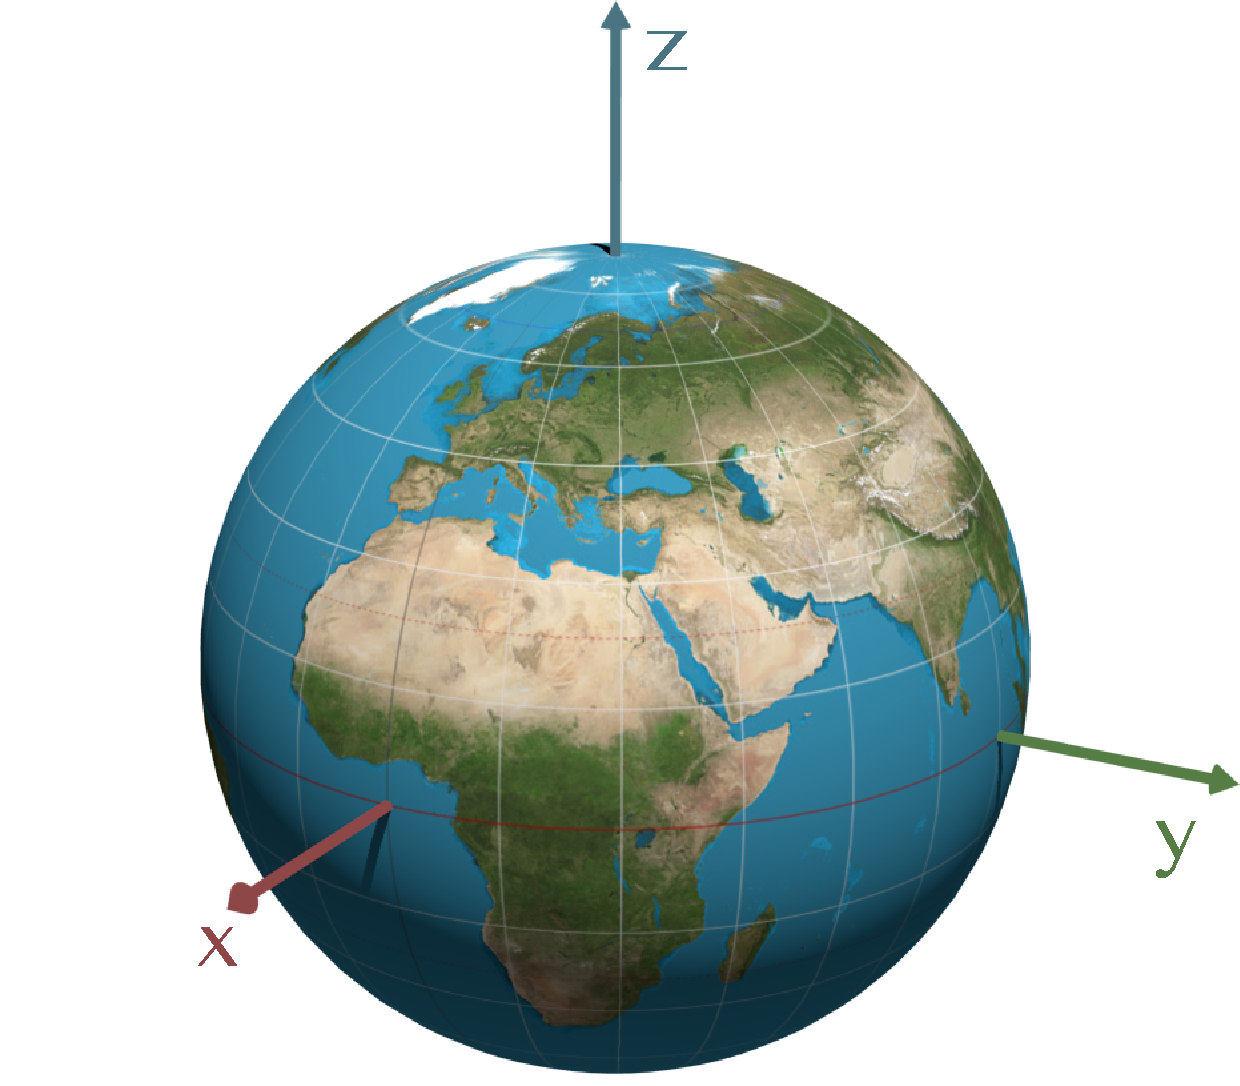
\includegraphics[scale=0.25]{figures/wgs84.pdf}
\caption{The WGS84 coordinate system and globe.}
\label{fig:wgs84}
\end{figure}

\subsection{Tesselating the Ellipsoid}

Triangle models are still the most common way of modeling renderable objects in 3D graphics softwares, even though other rendering techniques such as volumetric ray casting also is possible for terrain rendering (src).

A triangle mesh, or more generally a polygon mesh, is defined by a limited number of surface elements. This means that ellipsoids need to be approximated by some sort of tessellation or subdivision surface when modeled as a polygon mesh. There are several techniques for tessellating an ellipsoid. Some of them are covered in this section.

\subsubsection{Geographic Grid Tessellation}

Tessellating the ellipsoid using a geographic grid is a very straightforward approach. Ellipsoid vertex positions can be calculated using a transform from geographic coordinates to cartesian model space coordinates \cite[p. 25]{cozzi11}. Figure \ref{fig:tesselation_geo} shows three geographic grid tessellations of ellipsoids with constant number of latitudinal segments of 4, 8 and 16 respectively.

A common issue with geographic grids is something referred to as polar pinching. At both of the poles, segments will be pinched to one point which leads to an increasing amount of segments per area. This in turn results in oversampling in textures as well as possible visual artefacts in shading due to the very thin quads at the poles as well as possible performance penalties for highly tessellated globes.

\begin{figure}
    \centering
    \begin{subfigure}[b]{0.2\textwidth}
        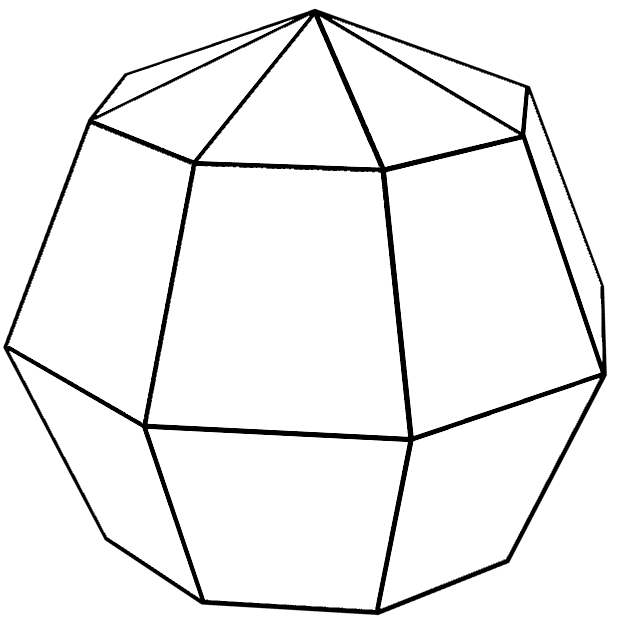
\includegraphics[width=\textwidth]{figures/tessellation/tessellation_geo1.png}
    \end{subfigure}
    ~ %add desired spacing between images, e. g. ~, \quad, \qquad, \hfill etc. 
      %(or a blank line to force the subfigure onto a new line)
    \begin{subfigure}[b]{0.2\textwidth}
        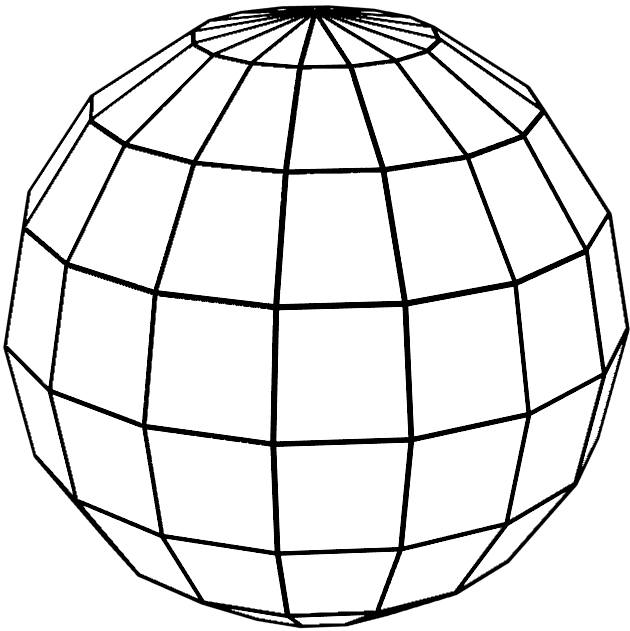
\includegraphics[width=\textwidth]{figures/tessellation/tessellation_geo2.png}
    \end{subfigure}
    ~ %add desired spacing between images, e. g. ~, \quad, \qquad, \hfill etc. 
    %(or a blank line to force the subfigure onto a new line)
    \begin{subfigure}[b]{0.2\textwidth}
        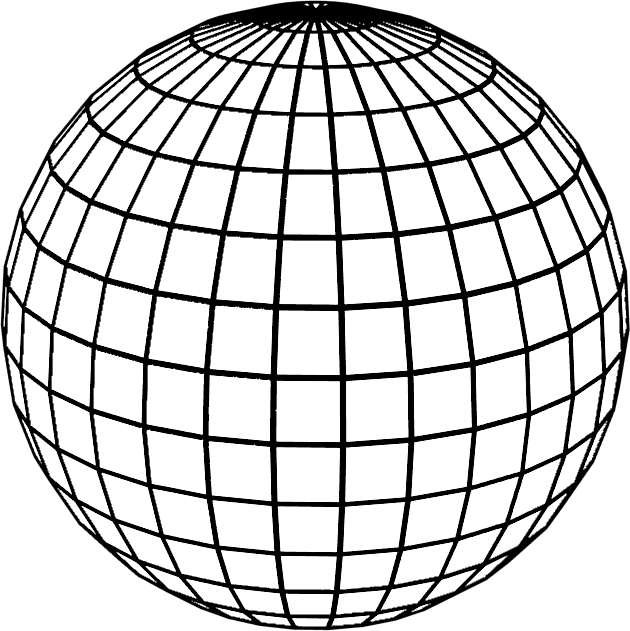
\includegraphics[width=\textwidth]{figures/tessellation/tessellation_geo3.png}
    \end{subfigure}
    \caption{Geographic grid tesselation.}
    \label{fig:tesselation_geo}
\end{figure}

\subsubsection{Quadrilateralized Spherical Cube Tessellation}
 
Another common tessellation method for spheres which can be generalized to ellipsoids is the quadrilateralized spherical cube tessellation. The standard approach is to subdivide a cube centered in the origin and then normalize the coordinates of all vertices to map them on a sphere. There are also other more complicated schemes designed to work with specific map projections \cite{dimi15}.

To model an ellipsoid from a sphere, the vertices can be linearly transformed with a scaling in the $x$, $y$, and $z$ directions individually. Figure \ref{fig:tesselation_cube} shows a tessellated spherical cube of four different detail levels.

\begin{figure}
    \centering
    \begin{subfigure}[b]{0.2\textwidth}
        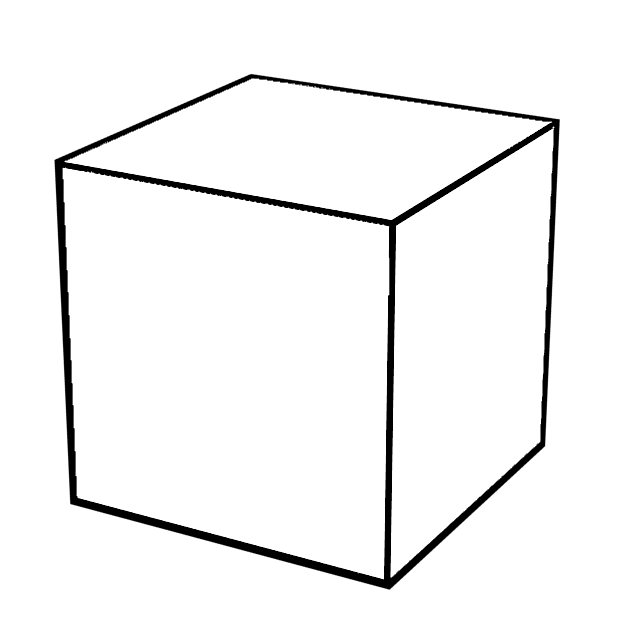
\includegraphics[width=\textwidth]{figures/tessellation/tessellation_cube1.png}
    \end{subfigure}
    ~ %add desired spacing between images, e. g. ~, \quad, \qquad, \hfill etc. 
      %(or a blank line to force the subfigure onto a new line)
    \begin{subfigure}[b]{0.2\textwidth}
        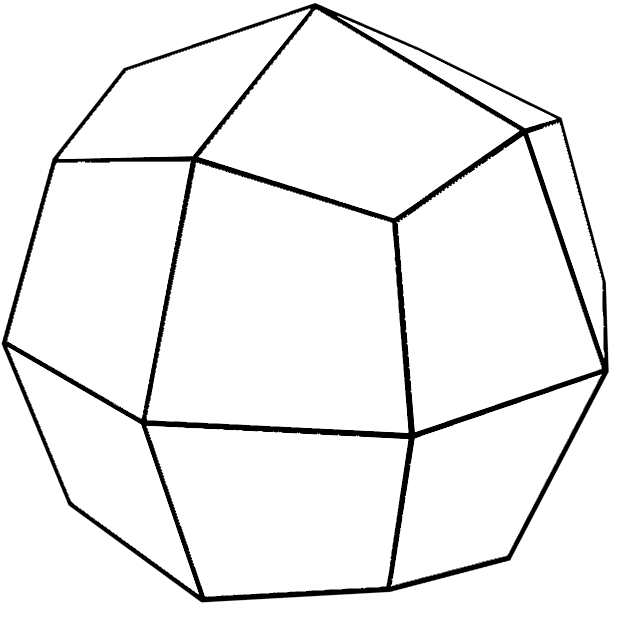
\includegraphics[width=\textwidth]{figures/tessellation/tessellation_cube2.png}
    \end{subfigure}
    ~ %add desired spacing between images, e. g. ~, \quad, \qquad, \hfill etc. 
    %(or a blank line to force the subfigure onto a new line)
    \begin{subfigure}[b]{0.2\textwidth}
        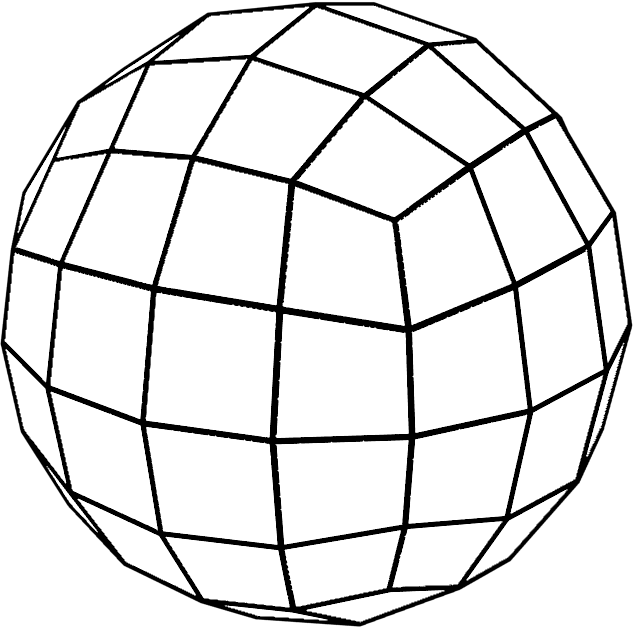
\includegraphics[width=\textwidth]{figures/tessellation/tessellation_cube3.png}
    \end{subfigure}
    ~ %add desired spacing between images, e. g. ~, \quad, \qquad, \hfill etc. 
    %(or a blank line to force the subfigure onto a new line)
    \begin{subfigure}[b]{0.2\textwidth}
        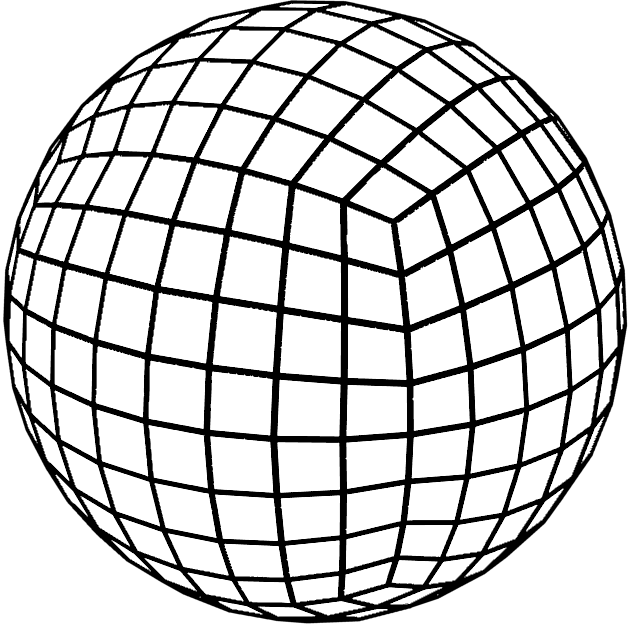
\includegraphics[width=\textwidth]{figures/tessellation/tessellation_cube4.png}
    \end{subfigure}
    \caption{Quadrilateralized spherical cube tessellation.}
    \label{fig:tesselation_cube}
\end{figure}

\subsubsection{Hierarchical Triangular Mesh}

The hierarchical triangular mesh (HTM) is a method of modeling the sky dome as a sphere proposed by astronomers in the Sloan Digital Sky Survey \cite{htm}. Instead of uniformly dividing cube faces, an alternative option is to subdivide a normalized octahedron by, in each subdivision step, split every triangle into four new triangles, see figure \ref{fig:tesselation_htm}. An ellipsoid can be created from the sphere by normalizing the coordinates and linearly rescaling them the same way that can be done for the spherical cube tessellation.

\begin{figure}
    \centering
    \begin{subfigure}[b]{0.2\textwidth}
        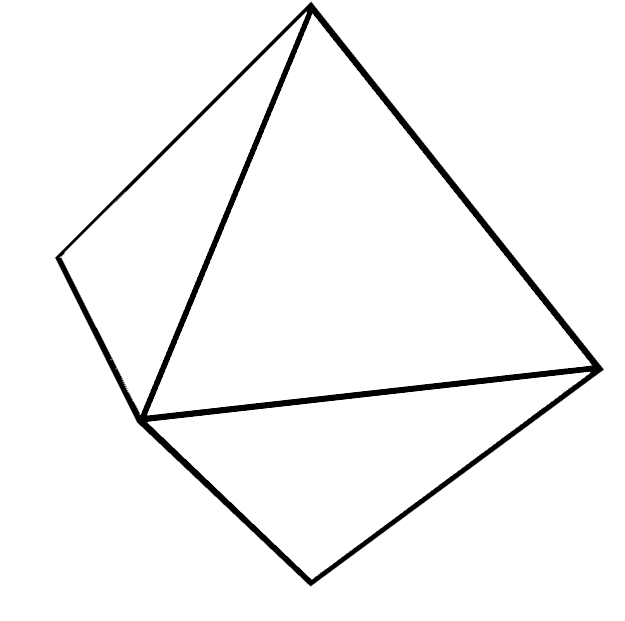
\includegraphics[width=\textwidth]{figures/tessellation/tessellation_htm1.png}
    \end{subfigure}
    ~ %add desired spacing between images, e. g. ~, \quad, \qquad, \hfill etc. 
      %(or a blank line to force the subfigure onto a new line)
    \begin{subfigure}[b]{0.2\textwidth}
        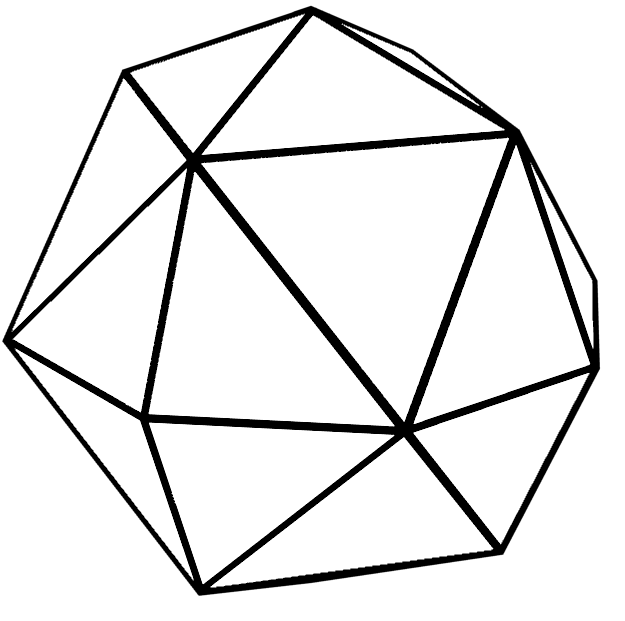
\includegraphics[width=\textwidth]{figures/tessellation/tessellation_htm2.png}
    \end{subfigure}
    ~ %add desired spacing between images, e. g. ~, \quad, \qquad, \hfill etc. 
    %(or a blank line to force the subfigure onto a new line)
    \begin{subfigure}[b]{0.2\textwidth}
        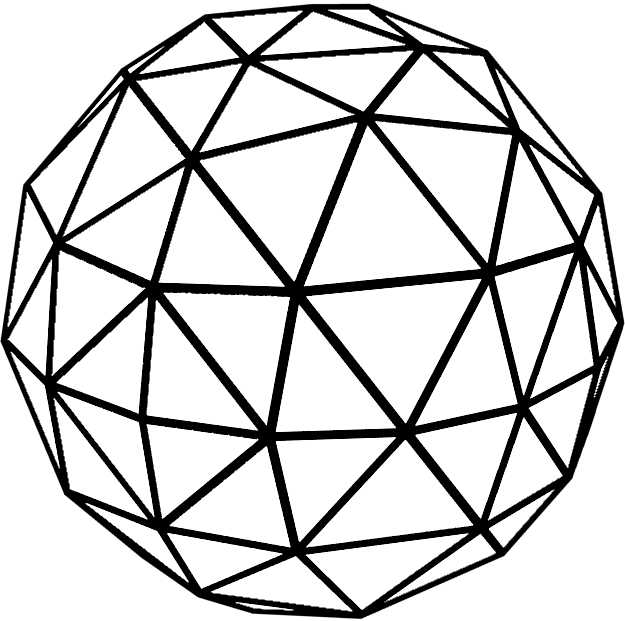
\includegraphics[width=\textwidth]{figures/tessellation/tessellation_htm3.png}
    \end{subfigure}
    ~ %add desired spacing between images, e. g. ~, \quad, \qquad, \hfill etc. 
    %(or a blank line to force the subfigure onto a new line)
    \begin{subfigure}[b]{0.2\textwidth}
        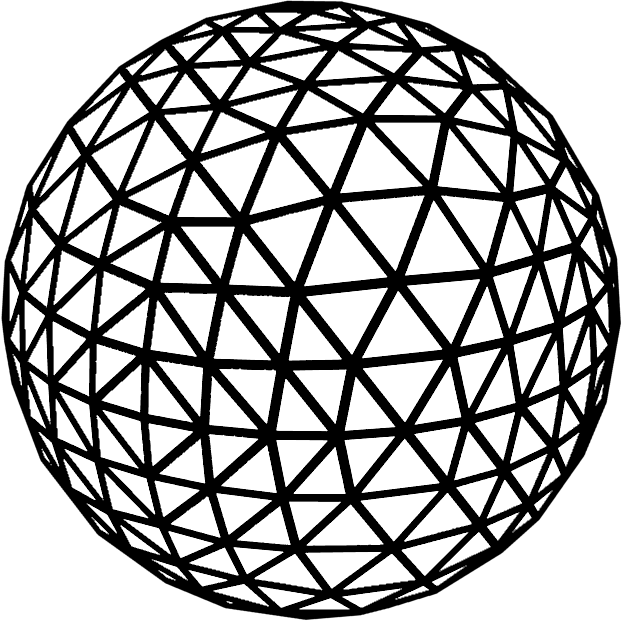
\includegraphics[width=\textwidth]{figures/tessellation/tessellation_htm4.png}
    \end{subfigure}
    \caption{Hierarchical triangular mesh tesselation.}
    \label{fig:tesselation_htm}
\end{figure}

\subsubsection{Hierarchical Equal Area IsoLatitude Pixelation}

Hierarchical Equal Area IsoLatitude Pixelation (HEALPix) is spherical tessellation scheme with corresponding map projection. The base level of the tessellation is built up of twelve quads, similar to a rhombic dodecahedron, which each can be subdivided further. The tessellation in figure \ref{fig:tesselation_healpix} shows how the vertices in the HEALPix tessellation leads to curvilinear quads.

\begin{figure}
    \centering
    \begin{subfigure}[b]{0.2\textwidth}
        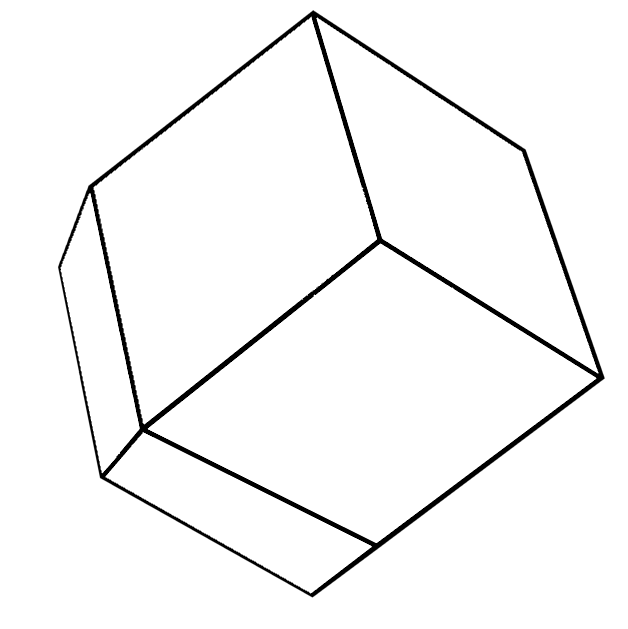
\includegraphics[width=\textwidth]{figures/tessellation/tessellation_healpix1.png}
    \end{subfigure}
    ~ %add desired spacing between images, e. g. ~, \quad, \qquad, \hfill etc. 
      %(or a blank line to force the subfigure onto a new line)
    \begin{subfigure}[b]{0.2\textwidth}
        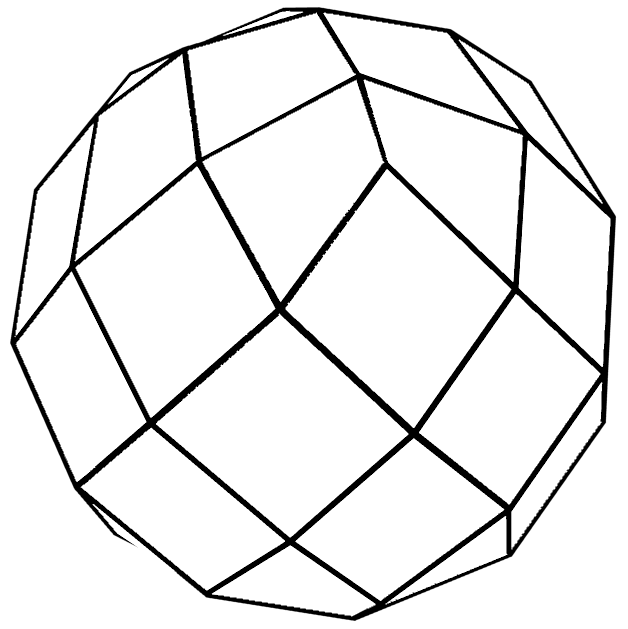
\includegraphics[width=\textwidth]{figures/tessellation/tessellation_healpix2.png}
    \end{subfigure}
    ~ %add desired spacing between images, e. g. ~, \quad, \qquad, \hfill etc. 
    %(or a blank line to force the subfigure onto a new line)
    \begin{subfigure}[b]{0.2\textwidth}
        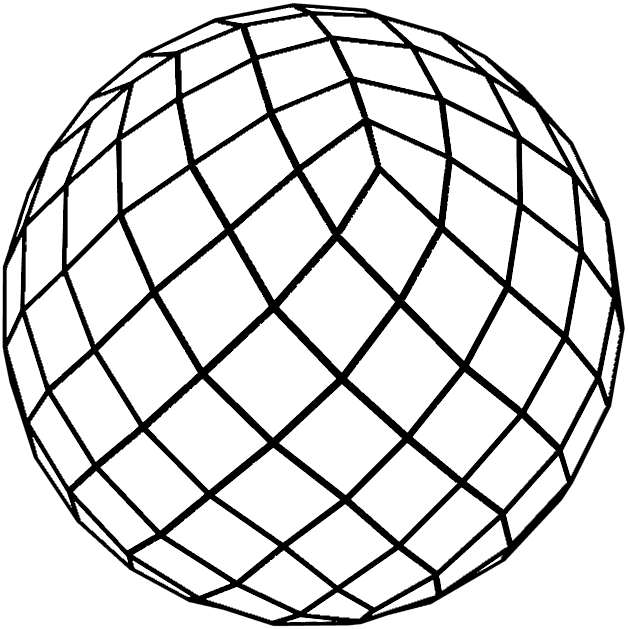
\includegraphics[width=\textwidth]{figures/tessellation/tessellation_healpix3.png}
    \end{subfigure}
    \caption{HEALPix tesselation.}
    \label{fig:tesselation_healpix}
\end{figure}

\subsubsection{Geographic Grid Tessellation With Polar Caps}

In their description of the ellipsoidal clipmaps method, Dimitrijevi\'{c} and Ran\v{c}i\'{c} introduces polar caps to avoid polar issues related to geographic grids \cite{dimi15}. The polar caps are simply used as a replacement of the problematic, oversampled regions around the poles. The caps can be modelled as grids projected onto the ellipsoid surface in their own georeferenced coordinate systems. One obvious issue with polar caps is the edge problem that occurs due to the fact that the caps are defined as separate meshes with vertices that do not coincide with the geographic vertices of the equatorial region, see figure caps. Dimitrijevi\'{c} and Ran\v{c}i\'{c} solves the issue by using a type of edge blending between the equatorial and polar segments \cite{dimi15}. Figure \ref{fig:tesselation_caps} shows a sphere tessellated with one equatorial region and two polar regions.

\begin{figure}
    \centering
    \begin{subfigure}[b]{0.2\textwidth}
        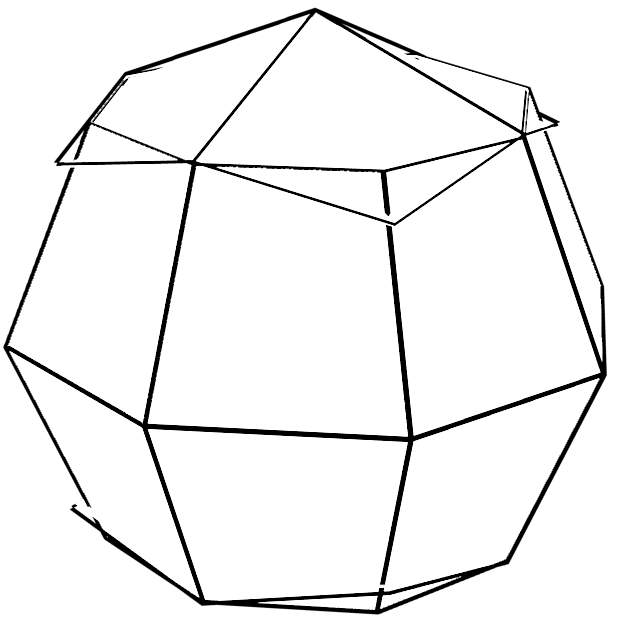
\includegraphics[width=\textwidth]{figures/tessellation/tessellation_caps_proj1.png}
    \end{subfigure}
    ~ %add desired spacing between images, e. g. ~, \quad, \qquad, \hfill etc. 
      %(or a blank line to force the subfigure onto a new line)
    \begin{subfigure}[b]{0.2\textwidth}
        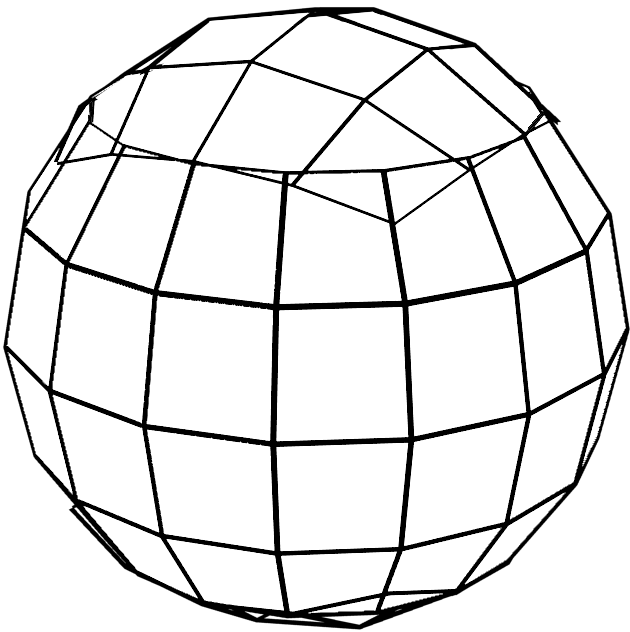
\includegraphics[width=\textwidth]{figures/tessellation/tessellation_caps_proj2.png}
    \end{subfigure}
    ~ %add desired spacing between images, e. g. ~, \quad, \qquad, \hfill etc. 
    %(or a blank line to force the subfigure onto a new line)
    \begin{subfigure}[b]{0.2\textwidth}
        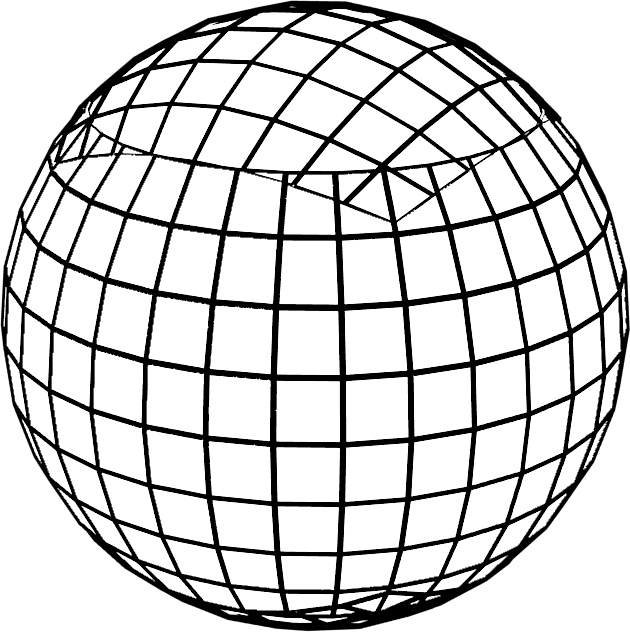
\includegraphics[width=\textwidth]{figures/tessellation/tessellation_caps_proj3.png}
    \end{subfigure}
    \caption{Geographic tessellation of an ellipsoid with polar caps.}
    \label{fig:tesselation_caps}
\end{figure}

\subsection{2D Parameterisation for Map Projections}

A map projection $P$ defines a transformation from cartesian model space coordinates to georeferenced (projected) coordinates, as in equation \ref{eq:proj}. The inverse projection $P^{-1}$ is used to find positions on the globe surface in model space given georeferenced coordinates as in equation \ref{eq:invproj}.

\begin{equation}
\label{eq:proj}
\begin{pmatrix} \phi  \\ \theta  \end{pmatrix}_{ georeferenced }=\vec { P } (x,y,z),
\end{equation}

\begin{equation}
\label{eq:invproj}
\begin{pmatrix} x \\ y \\ z \end{pmatrix}_{ modelspace }=\vec { P }^{-1} (\phi ,\theta ),
\end{equation}

Where $(x,y,z)^T$ is the cartesian coordinates of a point on the ellipsoid surface. The parameters $\phi$ and $\theta$ are georeferenced coordinates defining all positions on the globe. The georeferenced coordinates can have different definition range depending on which projection is used.

The globally positive gaussian curvature of any ellipsoid makes it impossible to unproject it on a flat 2D surface without any distortions. Different projections are used for different purposes. Equal-area projections preserve the size of a projected area as $\partial \phi \partial \theta / \partial \phi_0 \partial \theta_0 = 1$, while conformal projections preserve the shape of projected objects as $\partial \phi / \partial \theta = 1$; $\phi_0$ and $\theta_0$ are coordinates at the center of the projection with no distortion. No global projection can be both area-preserving and conformal \cite{dimi15}.

There are several possibilities for defining a coordinate transform for map projections. A common approach is to project the ellipsoid onto another shape that allows for being flattened out without distortion, such as a cube, a cylinder or a plane. These types of shapes are known as developable shapes and have zero gaussian curvature.

Choosing a map projection is tied together with the choice of ellipsoid tessellation. This is because the map often needs to be tiled up when rendering. Each tile has its local texture coordinate system which need to have a simple transform from the georeferenced coordinate system for texture sampling. If the tiles can be affinely transformed to the geo referenced coordinate system, texture sampling can be done on the fly; otherwise the geo referenced coordinates need to be reprojected which may be computationally heavy or impossible for real time applications.

The European Petroleum Survey Group (EPSG) has defined several standards for map projections of the Earth. Many of these are mentioned when discussing the different projections.

\subsubsection{Geographic Projections}

\begin{figure}[htbp]
    \centering
    \begin{subfigure}[bt]{0.4\textwidth}
        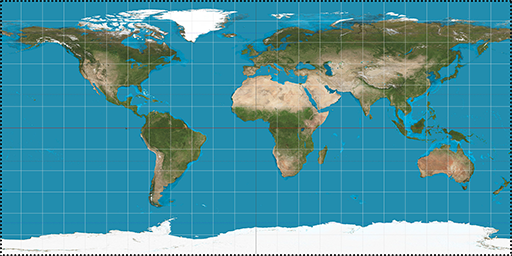
\includegraphics[width=\textwidth]{figures/developable_projected/equirectangular.png}
    \end{subfigure}
    \qquad
    \begin{subfigure}[bt]{0.15\textwidth}
        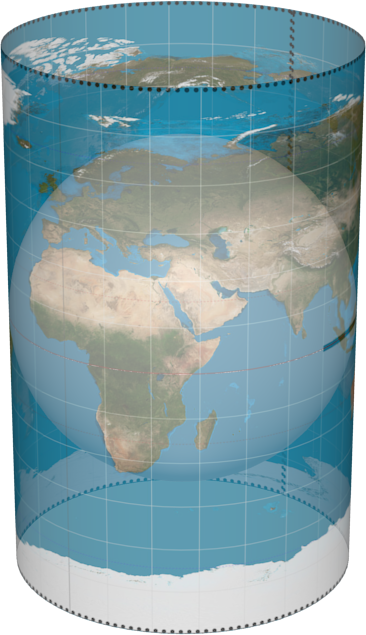
\includegraphics[width=\textwidth]{figures/map_projection/projection_geo.png}
    \end{subfigure}
    \caption{Geographic map projection.}
    \label{fig:proj_cube}
\end{figure}

\paragraph{Geocentric projection}
asd
\paragraph{Geodetic projection}
asd
\subsubsection{Geographic Projections}
asd
\subsubsection{Geographic Projections}
asd


\subsection{Dynamic Level of Detail}
Dynamic level of detail (LOD) is an important part in handling the extensive amount of data used in an out of core rendering software. The goal is to maximize the visual information on screen while minimizing the workload. In their book Rendering virtual 3D globes, Cozzi and Ring describes LOD rendering algorithms by three typical steps. \cite[p. 367]{cozzi11}

\begin{enumerate}
    \item Generation - Create versions at different level of detail of a model
    \item Selection - Choose a version based on some criteria or error metric (e.g., distance to object or the projected area it occupies on the screen)
    \item Switching - Transitions from one version to another in order to avoid noticing of the change in LOD known as popping artifacts.
\end{enumerate}

There are different types of LOD approaches for terrain rendering, and a suitable approach should be chosen based on characteristics of the terrain. Terrains can for example be restricted to being represented as height maps - a characteristic that can be exploited by the rendering algorithm. Cozzi and Ring describe the following three categories of LOD approaches: Discrete Level of Detail, Continuous Level of Detail and Hierarchical Level of Detail \cite[p. 368-371]{cozzi11}.

\subsubsection{Discrete Level of Detail}
In the Discrete Level Of Detail (DLOD) approach, multiple different representations of the terrain are created at different resolutions. DLOD is arguably the most simple LOD algorithm. It works not only for digital terrain models, but for arbitrary meshes. The set of terrain representations can either be predefined or generated using mesh simplification algorithms.

\begin{figure}[htbp]
    \centering
    \begin{subfigure}[bt]{0.9\textwidth}
        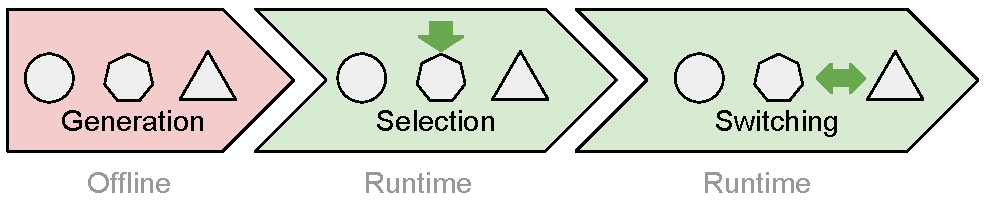
\includegraphics[width=\textwidth]{figures/lod/lod_overview.pdf}
    \end{subfigure}
    \caption{DLOD. Generate offline, select and switch at runtime.}
    \label{fig:lod}
\end{figure}

\begin{figure}
    \centering
    \begin{subfigure}[b]{0.2\textwidth}
        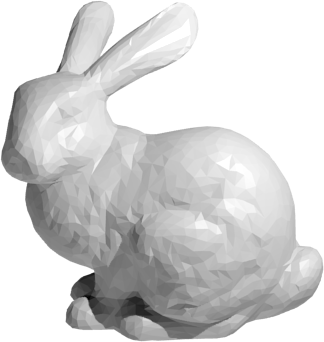
\includegraphics[width=\textwidth]{figures/lod/decimation1.png}
    \end{subfigure}
    ~ %add desired spacing between images, e. g. ~, \quad, \qquad, \hfill etc. 
      %(or a blank line to force the subfigure onto a new line)
    \begin{subfigure}[b]{0.2\textwidth}
        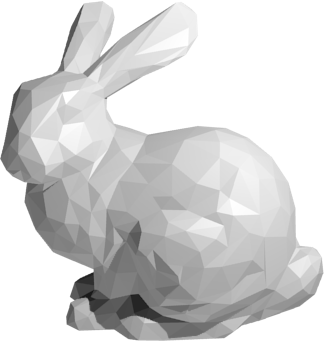
\includegraphics[width=\textwidth]{figures/lod/decimation2.png}
    \end{subfigure}
    ~ %add desired spacing between images, e. g. ~, \quad, \qquad, \hfill etc. 
    %(or a blank line to force the subfigure onto a new line)
    \begin{subfigure}[b]{0.2\textwidth}
        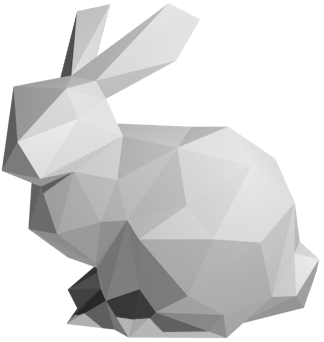
\includegraphics[width=\textwidth]{figures/lod/decimation3.png}
    \end{subfigure}
    \caption{A range of predefined meshes with decreasing resolution}
    \label{fig:dlod}
\end{figure}

At run time, the main objective is to select one (or generate) a suitable representation. This approach does not provide any means of dealing with large scale datasets, which makes it unsuitable for globe rendering (ref virtual globes).

\subsubsection{Continuous Level of Detail}
The continuous LOD (CLOD) approach represents a model in a way that allows the resolution to be selected arbitrary. This is usually implemented by a base mesh combined with a sequence of operations that successively changes the level of detail of the model. Two typical such operations are ``edge collapse'' (removes two triangles from the mesh) and its inverse, ``vertex split'' (adds two triangles to the mesh). 

\begin{figure}
    \centering
    \begin{subfigure}[b]{0.2\textwidth}
        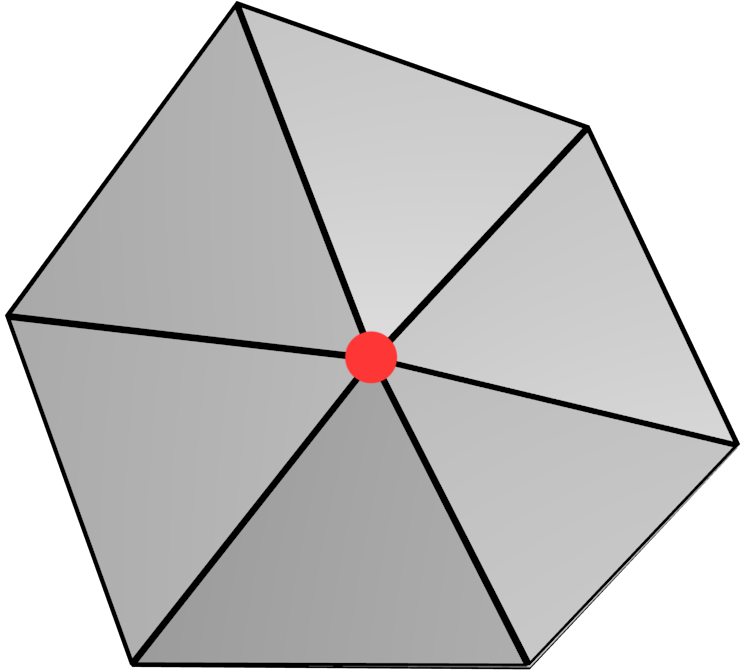
\includegraphics[width=\textwidth]{figures/lod/vertex_split1.png}
    \end{subfigure}
    ~ %add desired spacing between images, e. g. ~, \quad, \qquad, \hfill etc. 
      %(or a blank line to force the subfigure onto a new line)
    \begin{subfigure}[b]{0.2\textwidth}
        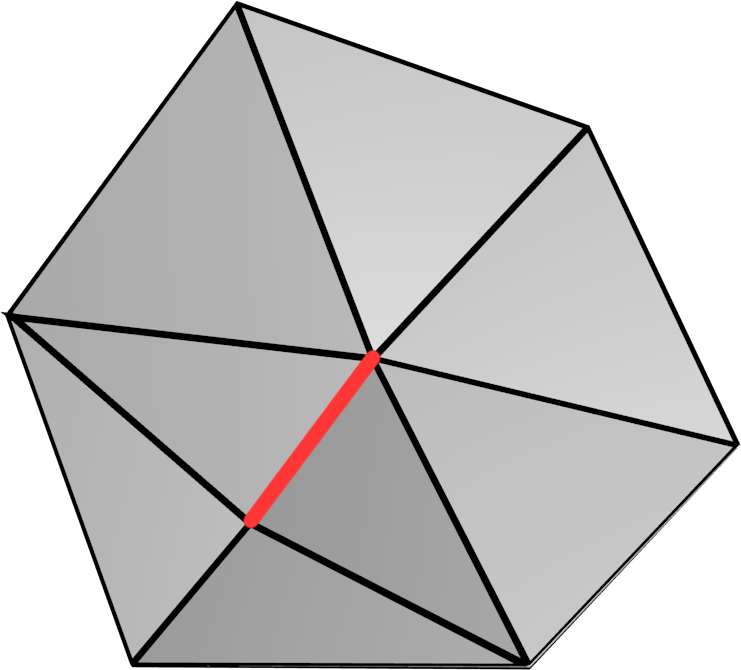
\includegraphics[width=\textwidth]{figures/lod/vertex_split2.png}
    \end{subfigure}
    \caption{Edge collapse in continous LOD}
    \label{fig:clod}
\end{figure}

According to Cozzi and Ring \cite[p. 368]{cozzi11} CLOD has previously been the most popular approach for rendering terrain at interactive rates, with implementations such as Real-time Optimally Adaptive Mesh (ROAM). The main reason CLOD algorithms are not widely employed these days is due to the increase in triangle throughput on modern GPUs, causing the CLOD operations done on the CPU in many cases to act as a bottleneck for the rendering time.

A special branch of CLOD worth mentioning is the so called infinite LOD. In this approach the terrain is represented by a mathematical function - an implicit surface. These functions can be defined by fractal algorithms and produce complex characteristics, or they can define simple geometric shapes such as spheres or ellipsoids. As every point on these types of surfaces are precisely defined, triangle meshes can be generated with no limit on the level of detail. This approach is not suitable for incorporating real world data, but it is used by terrain engines such as Outerra and Terragen to procedurally generate terrain at any desired level of detail \cite{outerraprocedural09}. 

\subsubsection{Hierarchical Level of Detail}
Hierarchical Level of Detail (HLOD) can be seen as a generalization of DLOD. HLOD algorithms operates on hierarchically arranged, predefined chunks of the full model. Each chunk is processed, stored and rendered separately. By doing this, HLOD approaches tackles the weaknesses of CLOD, essentially by doing the following.

\begin{enumerate}
    \item Reduce processing time on CPU: The only CPU task that HLOD algorithms has to deal with during runtime is to select a suitable subset of the predefined chunks for rendering. This is a relatively fast procedure in contrast to iteratively applying changes to the raw geometry, as done in CLOD.
    \item Reduce the data traffic to GPU: Data is uploaded to the GPU in larger batches but not very often, since the data is static and GPU caching can be done. With CLOD, the geometry data is updated on a per-frame basis, and can't be cached on the GPU. Being able to perform GPU caching allow HLOD to better minimize the traffic to the GPU.
\end{enumerate}

HLOD uses spatial hierarchical data structures such as quadtrees or octrees for storing the chunk data. The root node of the tree holds a full representation of the model at its lowest level of detail a one single chunk. At successive levels, the model is represented at a higher level of detail but divided up into several chunks. This concept is illustrated in figure hlod.

\begin{figure}[htbp]
    \centering
    \begin{subfigure}[bt]{0.4\textwidth}
        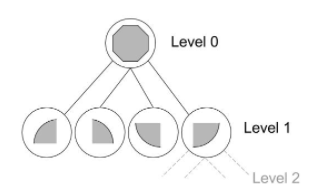
\includegraphics[width=\textwidth]{figures/lod/hlod_tmp.png}
    \end{subfigure}
    \caption{HLOD using a quadtree.}
    \label{fig:hlod}
\end{figure}

Generally, selecting all the chunks at a specific level in the tree yields a complete representation of the model. Furthermore, chunks may be selected from different levels for different parts of the model and still yield a full representation of the model. This allows for view dependent rendering of the model. Algorithm chunk selection describes pseudo code for recursively rendering the full model at view dependent level of detail.

\begin{algorithm}[htp]
  \SetKwFunction{RenderLOD}{}
  \SetKwProg{myalg}{RenderLOD}{}{}
  \myalg{\RenderLOD{Camera C, ChunkNode N}}{
  \eIf{ErrorMetric($C$, $N$) < threshold}{
        Render($N$, $C$)
    }{
        \For{$child$ \textbf{in} $children(N)$}{
            RenderLOD($child$, $C$)
        }
    }
  }{}
  \caption{Algorithm with procedure}
\end{algorithm} 


This example uses a depth first approach for rendering of chunks. Other common schemes for traversing the hierarchy are breadth first and inverse breadth first.

The algorithm traverses the tree and calculates an error metric at each node with respect to the current camera position. If the calculated error is larger than a certain threshold, the algorithm recursively repeats the procedure for all the chunk's children, which has higher level of detail. This general scheme can be used for rendering one-dimensional curves (using a binary tree structure), two-dimensional surfaces (using a quadtree) or volumes (using an octree).

Another key feature of HLOD as opposed to DLOD and CLOD is that it can naturally be integrated with out-of-core rendering, as chunks can be loaded into memory on-demand and thrown away when not needed.




